\documentclass{article}%
\usepackage[T1]{fontenc}%
\usepackage[utf8]{inputenc}%
\usepackage{lmodern}%
\usepackage{textcomp}%
\usepackage{lastpage}%
\usepackage[head=40pt,margin=0.5in,bottom=0.6in]{geometry}%
\usepackage{graphicx}%
%
\title{\textbf{Carlos Prosperi denunció llegada de médicos palestinos al Hospital Vargas}}%
\author{EL NACIONAL}%
\date{07/03/2019}%
%
\begin{document}%
\normalsize%
\maketitle%
\textbf{URL: }%
http://www.el{-}nacional.com/noticias/sociedad/carlos{-}prosperi{-}denuncio{-}llegada{-}medicos{-}palestinos{-}hospital{-}vargas\_273740\newline%
%
\textbf{Periodico: }%
EN, %
ID: %
273740, %
Seccion: %
Sociedad\newline%
%
\textbf{Palabras Claves: }%
NO\_TIENE\newline%
%
\textbf{Derecho: }%
2.1%
, Otros Derechos: %
\newline%
%
\textbf{\textit{El diputado aseguró que este personal no maneja el idioma español}}%
\newline%
\newline%
%
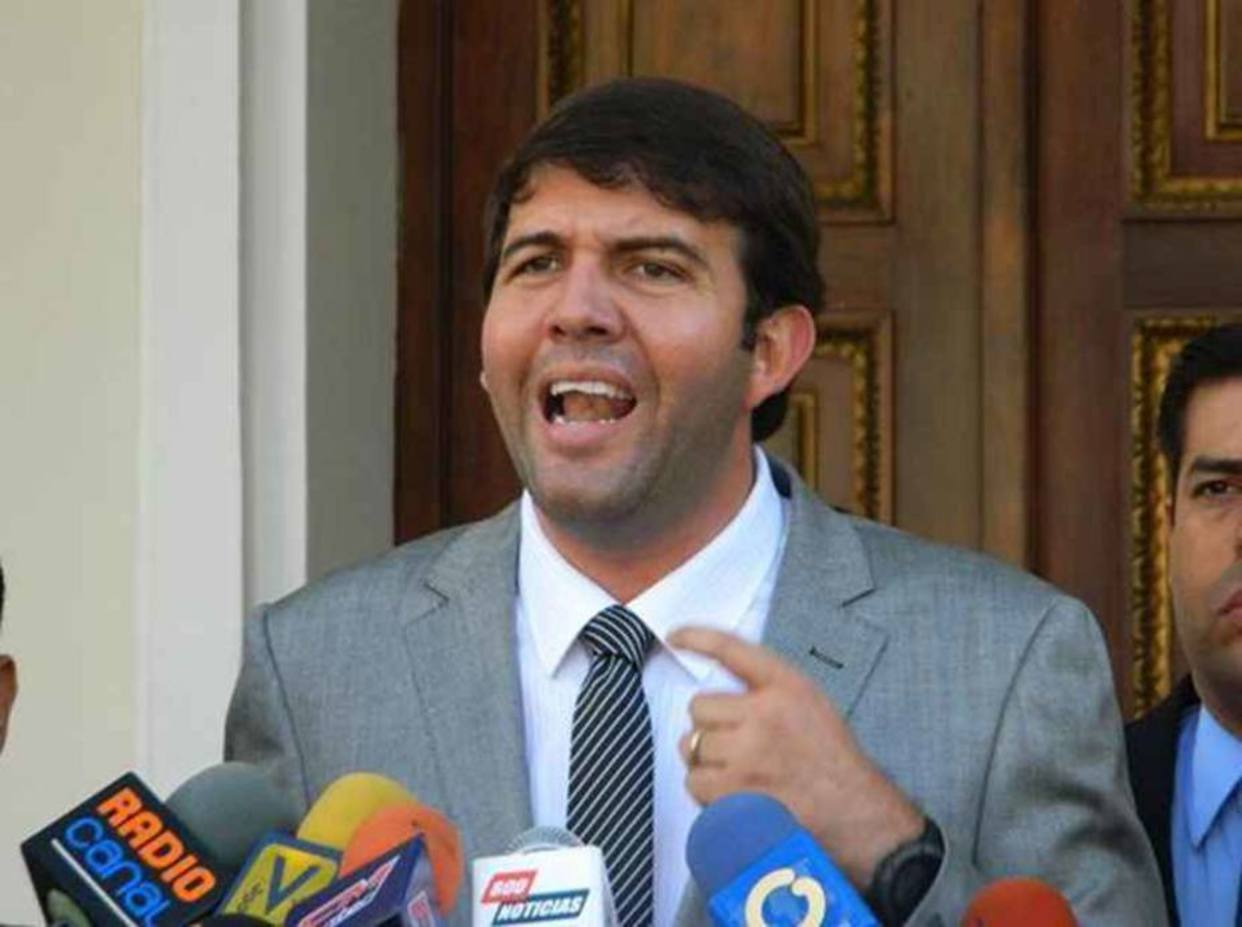
\includegraphics[width=300px]{EN_273740.jpg}%
\newline%
%
Carlos Prosperi, diputado a la Asamblea Nacional (AN) por el estado Guárico, denunció la llegada de una serie de médicos palestinos al Hospital José María Vargas, en Caracas.%
\newline%
%
“Lo más preocupante de estos médicos es que ni siquiera hablan nuestro idioma. Quien se dirige a otro país a laborar en el ámbito de la salud debe tener nivel avanzado del idioma de ese país”, denunció el parlamentario.%
\newline%
%
Prosperi aseguró que seis de los médicos ya se encuentran trabajando en el Hospital Vargas y otro grupo en el Materno de Macuto.%
\newline%
%
“No sabemos dónde adquirieron el título de su especialidad. No mostraron ningún tipo de expediente”, recalcó.%
\newline%
%
El parlamentario aseguró que en Venezuela hay personal calificado para cubrir las necesidades de los centros de salud.%
\newline%
%
\end{document}